

\documentclass[twoside]{article}
\usepackage{amsmath}
\usepackage{amssymb}
\usepackage{hyperref}
\usepackage{graphicx}
\usepackage{listings}
\hypersetup{
    colorlinks=true,
    linkcolor=blue,
    filecolor=magenta,      
    urlcolor=cyan,
}
\usepackage{geometry}
\setlength{\oddsidemargin}{0.25 in}
\setlength{\evensidemargin}{-0.25 in}
\setlength{\topmargin}{-0.9 in}
\setlength{\textwidth}{6.5 in}
\setlength{\textheight}{8.5 in}
\setlength{\headsep}{0.75 in}
\setlength{\parindent}{0 in}
\setlength{\parskip}{0.1 in}

\newcommand{\x}{{\bf x}}
\newcommand{\w}{{\bf w}}
\newcommand{\q}{{\bf q}}
\newcommand{\br}{{\bf r}}
\newcommand{\bP}{{\bf P}}
\newcommand{\on}{\operatorname}
\newcommand{\E}{\on{E} }
\newcommand{\vpi}{\mathbf{v}_{\pi}}
\newcommand{\rpi}{\mathbf{r}_{\pi}}
\newcommand{\Ppi}{\mathbf{P}_{\pi}}
\newcommand{\W}{\bf{W}}
\newcommand{\sol}{\leftskip50pt\rightskip50pt\parindent0em}
\newcommand{\en}{\vskip\baselineskip\vspace{-1cm}}
\title{Assignment 1 for CMPUT 652 RL with Robots}


\begin{document}

\maketitle

Total 110 points. Complete  within the given space using \LaTeX ~or handwritten notes. Show the derivations or the steps for obtaining partial points. On the other hand, mistakes, missteps or bad reasoning behind a correct answer will result in points deducted. Submit at armahmood@ualberta.ca

\newpage

\section{\normalsize 
Consider the supervised regression problem of predicting an output $Y$ from a vector input $\bf x$ using a linear function with a vector parameter $\bf w$. We found in the lecture that the Mean Squared Error (MSE) $\E\left[ \left( Y - \x^\top\w \right)^2 \right]$ is a reasonable objective for this problem.
Derive the Least-Squares (LS) method, defined below, from MSE (5 points).
}
\begin{align}
\w^{\on{LS}}_{t+1} &= \left( \frac{1}{t} \sum_{k=1}^t \x_k \x_k^\top \right)^{-1} \left( \frac{1}{t} \sum_{k=1}^t \x_k Y_k \right).
\end{align}

\begin{align*}
	\E\left[ \left( Y - \x^\top\w \right)^2 \right] &= \E \left[ Y^2 + \w^\top\x\x^\top\w - 2\w^\top\x Y \right] \\
	&= \E\left[Y^2\right] + \w^\top\E\left[\x\x^\top \right]\w - 2\w^\top\E\left[\x Y \right]
\end{align*}
{\sol
The exact solution can be obtained by setting the derivative equal to 0 and the Least-Square solution can be obtained by substituting the expected values with sample average:

}
\en
\begin{align*} 
	\nabla_{\w}\E\left[ \left( Y - \x^\top\w \right)^2 \right] &= 2\E\left[\x\x^\top \right]\w - 2\E\left[\x Y \right] = 0 \\
	\w^* &= \E\left[\x\x^\top\right]^{-1}\E\left[\x Y\right]\\
	\w^{\on{LS}}_{t+1} &= \left( \frac{1}{t} \sum_{k=1}^t \x_k \x_k^\top \right)^{-1} \left( \frac{1}{t} \sum_{k=1}^t \x_k Y_k \right)
\end{align*}


%\vspace{1cm}
\section{\normalsize 
Continuing with the supervised regression problem, derive the Stochastic Gradient Descent (SGD) method, defined below, from MSE (5 points).
}
\begin{align}
\w_{t+1} &= \w_{t} + 2 \alpha_t \left( Y_t - \x_t^\top \w_t \right) \x_t.
\end{align}

\begin{align*}
\E\left[ \left( Y - \x^\top\w \right)^2 \right] &= \E \left[ Y^2 + \w^\top\x\x^\top\w - 2\w^\top\x Y \right] \\
&= \E\left[Y^2\right] + \w^\top\E\left[\x\x^\top \right]\w - 2\w^\top\E\left[\x Y \right]
\end{align*}
{\sol
Stochastic Gradient Descent can be obtained from approximate the exact gradient with one sample:

}
\en
\begin{align*}
\nabla_{\w}\E\left[ \left( Y - \x^\top\w \right)^2 \right] &= 2\E\left[\x\x^\top \right]\w - 2\E\left[\x Y \right] \\
&\approx 2\left(\x_t\x_t^\top\w-\x_tY_t \right)\\
&\approx -2\left(Y_t - \x_t^\top\w_t\right)\x_t\\
\w_{t+1} &= \w_{t} + 2 \alpha_t \left( Y_t - \x_t^\top \w_t \right) \x_t
\end{align*}

 \newpage
\section{\normalsize 
According to the strong law of large numbers, sample mean is a consistent estimator of the expected value (See Lemma 3, pg 18, of \href{https://era.library.ualberta.ca/files/cbc386j54q/Mahmood_Ashique_201709_PhD.pdf}{Mahmood 2017}). Use this fact to argue that the sample MSE $\frac{1}{t} \sum_{k=1}^t \left( Y_k - \x_k^\top\w \right)^2$ objective is a consistent estimator of MSE (5 points).
}

\begin{align*}
\E\left[ \left( Y - \x^\top\w \right)^2 \right] &= \E \left[ Y^2  - 2\w^\top\x Y + \w^\top\x\x^\top\w\right] \\
&= \E\left[Y^2\right]  - 2\w^\top\E\left[\x Y \right] + \w^\top\E\left[\x\x^\top \right]\w\\
\frac{1}{t} \sum_{k=1}^t \left( Y_k - \x_k^\top\w \right)^2 &=\frac{1}{t} \sum_{k=1}^t \left(Y_k^2  - 2\w^\top\x_k Y_k + \w^\top\x_k\x_k^\top\w\right)\\
&=\frac{1}{t} \sum_{k=1}^t Y_k^2 - 2\w^\top\frac{1}{t} \sum_{k=1}^t \x_k Y_k +\w^\top\frac{1}{t} \sum_{k=1}^t(\x_k\x_k^\top) \w
\end{align*}
{\sol
From above, the three terms of sample mean in sample MSE are consistent estimators of the three terms of expected value in MSE. Based on the fact that the sum of consistent estimators is still consistent, the sample MSE objective is a consistent estimator of MSE.
	
}
\en


\vspace{1cm}

\section{\normalsize 
Similarly, argue that LS is a consistent estimator of the solution to MSE (5 points).
}

{\sol
From Q1, we can directly write out the form of solutions obtained from MSE and LS:

}
\en
\begin{align*}
	\w^{\on{MSE}} &= \E\left[\x\x^\top\right]^{-1}\E\left[\x Y\right]\\
	\w^{\on{LS}}_{t+1} &= \left( \frac{1}{t} \sum_{k=1}^t \x_k \x_k^\top \right)^{-1} \left( \frac{1}{t} \sum_{k=1}^t \x_k Y_k \right)
\end{align*}

{\sol
From above, the two terms of sample mean from LS are consistent estimators of the two terms of expected value from MSE. Based on the fact, the multiplication of consistent estimators is still consistent, LS is a consistent estimator of the solution of MSE.

}
\en
\newpage

\section{\normalsize 
Establish a relationship between MSE and the following: $\E_{\x}\left[ \left( \E_{Y|{\x}}\left[ Y\right] - \x^\top\w \right)^2 \right]$.
Note that MSE can be written as $\E\left[ (Y - \x^\top \w)^2 \right] = \E_{\x}\E_{Y|{\x}}\left[ (Y - \x^\top \w)^2 \right]$. Also, the expectations $\E_{X}$ and $\E_{Y|X}$ can be elaborated as $\E_{X} f(X) = \int_{\mathcal{X}} p^*(x) f(x) dx$ and $E_{Y|X} f(Y) = \int_{\mathcal{Y}} p^*(y|x) f(y) dy$
(5 points).
}

\begin{align*}
	\E\left[ (Y - \x^\top \w)^2 \right] &= \E_{\x}\E_{Y|{\x}}\left[ (Y - \x^\top \w)^2 \right]\\
	&=\int_{\mathcal{X}} p^*(x) \int_{\mathcal{Y}} p^*(y|x) (y - x^\top \w)^2 dy dx\\
	&=\int_{\mathcal{X}} p^*(x) \int_{\mathcal{Y}} p^*(y|x) y^2 - 2yx^\top\w + \w^\top xx^\top \w dy dx\\
	&=\int_{\mathcal{X}} p^*(x) \left[\E_{Y|\x}\left[Y^2\right] -2\E_{Y|\x}\left[Y\right]\x^\top\w+ \w^\top xx^\top \w \right]dx\\
	&=\int_{\mathcal{X}} p^*(x) \left[\E_{Y|\x}\left[Y\right]^2 -2\E_{Y|\x}\left[Y\right]\x^\top\w+ \w^\top xx^\top \w \right]dx\\
	&\text{ the fact that $Y$ is independent with itself given $\x$ is used}\\
	&=\int_{\mathcal{X}} p^*(x) \left( \E_{Y|{\x}}\left[ Y\right] - \x^\top\w \right)^2 dx\\
	&=\E_{\x}\left[ \left( \E_{Y|{\x}}\left[ Y\right] - \x^\top\w \right)^2 \right]
\end{align*}


%\vspace{1cm}

\section{\normalsize 
Objective functions serve many purposes. They bring specificity to the problem formulation, provide a criteria for evaluation and can be used as a basis for deriving new algorithms. 
Accordingly, the same problem may have different associated objectives.
For example, the sample MSE is widely used to evaluate the performance of a learning method, but not all methods ensue from MSE.
Consider the following objective $\on{MSE}_{\on L2}$, which is a slight modification to MSE: $\on{MSE}_{\on L2}(\w) = \E\left[ \left( Y - \x^\top \w \right)^2 + \lambda \w^\top \w \right]$.
Derive the following method know as ridge regression from $\on{MSE}_{\on L2}$
(5 points).
}
\begin{align}
\w^{\on{RR}}_{t+1} = \left( \frac{1}{t} \sum_{k=1}^t \x_k \x_k^\top + \lambda {\bf I} \right)^{-1} \left( \frac{1}{t} \sum_{k=1}^t \x_k Y_k \right), \text{ where $\bf I$ is the identity matrix}.
\end{align}
$$
\on{MSE}_{\on L2}(\w) = \E\left[ Y^2 -2Y\x^\top\w + \w^\top \x\x^\top \w + \lambda \w^\top \w \right]
$$
{\sol
$\w$ can be solved by setting the derivative equal to 0 and the required result can be obtained by substituting the expected value with sample average:

}
\en
\begin{align*}
	\nabla_{\w}\on{MSE}_{\on L2}(\w) &= \E\left[-2\x Y + 2 \x\x^\top \w + 2\lambda \w \right] = 0\\
	\E\left[\x Y\right] &= \E\left[\x\x^\top +\lambda\bf{I} \right]\w\\
	\w &=\E\left[\x\x^\top +\lambda\bf{I} \right]^{-1}\E\left[\x Y\right]\\
	\w^{\on{RR}}_{t+1} &= \left( \frac{1}{t} \sum_{k=1}^t \x_k \x_k^\top + \lambda {\bf I} \right)^{-1} \left( \frac{1}{t} \sum_{k=1}^t \x_k Y_k \right)
\end{align*}



\newpage

\section{\normalsize 
Relate the MSE objective for supervised regression to the cross-entropy objective: $\on{CE}(\w) = -\int_{\mathcal{X}} p^*(x) \int_{\mathcal{Y}} p^*(y|x) \log p_{\w}(y|x) dy dx$, where $p^*$ is the true distribution of $Y$ and $\x$, and $ p_{\w}$ is the estimated distribution.
Use the fact that \\
$\on{MSE}(\w) = \E\left[ \left(Y - \x^\top \w \right)^2 \right] = \int_{\mathcal{X}} p^*(x) \int_{\mathcal{Y}} p^*(y|x) (y - x^\top \w)^2  dy dx$.
 (5 points).
}
{\sol
The relation can be built if we assume $p$ here is a Gaussian distribution and $\w$ is the weight of a linear model:

}
\en

\begin{align*}
	p_\w(y|x) &= \frac{1}{\sqrt{2\pi}\sigma}\exp\left(-\frac{(y-x^\top\w)^2}{2\sigma^2} \right)\\
	\log p_\w(y|x) &= -\frac{(y-x^\top\w)^2}{2\sigma^2}-\log \sqrt{2\pi}\sigma
\end{align*}
{\sol
If we insert $\log p_\w(y|x)$ in the CE objective, it will have the same form as MSE objective except the constant term:
	
}
\en
\begin{align*}	
	\on{CE}(\w) &= -\int_{\mathcal{X}} p^*(x) \int_{\mathcal{Y}} p^*(y|x) \left( -\frac{(y-x^\top\w)^2}{2\sigma^2}-\log \sqrt{2\pi}\sigma\right) dy dx\\
	\on{CE}(\w) &= \log \sqrt{2\pi}\sigma - \frac{1}{2\sigma^2}\int_{\mathcal{X}} p^*(x) \int_{\mathcal{Y}} p^*(y|x) \left( -(y-x^\top\w)^2\right) dy dx\\
\end{align*}

%\vspace{7cm}

\section{\normalsize 
We discussed how supervised and reinforcement learning problems are fundamentally different.
Show how that difference impacts the choice of policy optimization objective in terms of cross entropy in the case of bandits.
More specifically, formulate the policy optimization problem with a cross entropy objective, discuss the difference between this objective and the cross entropy objective for supervised regression defined above, and relate this difference to the fundamental difference between supervised and reinforcement learning problems
 (5 points).
}
{\sol
To build the objective, we can use a Cross Entropy objective of the following form: $\on{CE}(\pi_\theta, \pi^*) = -\int_\mathcal{A} \pi_\theta(a) \log \pi^*(a)\, da$, where $ \pi_\theta, \pi^* $ are current policy and optimal policy respectively. The relationship can be established with a Boltzman distribution $Z^{-1} e^{q(a) \tau^{-1}}$, where$Z$ is a normalizing constant and $\tau$ is called the \textit{temperature}, which controls the entropy of the distribution. In this case, the objective can be written as:

}
\en

\begin{align*}
	-\arg\min_\theta \int_\mathcal{A} \pi_\theta(a) \log \pi^*(a)\, da &= -\arg\min_\theta \int_\mathcal{A} \pi_\theta(a) \log Z^{-1} e^{q(a) \tau^{-1}}\, da \\
	&= -\arg\min_\theta\int_\mathcal{A} \pi_\theta(a)( \tau^{-1} q(a) - \log Z) \, da\\
	&= -\arg\min_\theta \int_\mathcal{A} \pi_\theta(a) q(a) \, da
\end{align*}
{\sol
The difference is xxxxxxxxxxxxxxxxxxxxxxxxxxx xxxxxxxxxxxxxxxxxxxxxxxxxxxxxxxxxx xxxxxxxxxxxxxxxxxxxxxxxxxxxxxxxx xxxxxxxxxxxxxxxxxxxxxxxx xxxxxxxxxxxxxxxxxxxxxxxxxxxxxxxxxxx xxxxxxxxxxxxxxxxxxxxxxxxxxxxxxxxxxx xxxxxxxxxxxxxxxx

}
\en


\newpage
\section{\normalsize 
The expected policy gradient update for contextual bandit problem can be given as follows: $\E\left[ - \log \pi_\theta\left( A | X \right) R \right]$, where $X$ is a given context, $\pi_\theta$ is the parameterized policy distribution maintained by the agent, $A$ is the action chosen by the agent according to $\pi_\theta$, and $R$ is the subsequent reward.
Show that this update can be derived by calculating the gradient of the cross entropy objective: $\on{CE}(\theta) = - \int_{\mathcal{X}} p(x) \int_{\mathcal{A}} \pi_\theta(a|x) \log \pi^*(a|x) da dx  $, where $p$, which is not a function of $\theta$, is the distribution of context $X$. Also, $\pi^*$ is the ideal policy distribution defined as the Boltzmann distribution $\pi^*(a|x) = Z^{-1} e^{q(x,a) \tau^{-1}}$, where $q(x,a) = \E\left[ R | A = a, X = x \right]$ is the contextual action value.
 (10 points).
}
{\sol
Similar to Q8, we insert the Boltzman distribution $\pi^*(a|x) = Z^{-1} e^{q(x, a) \tau^{-1}}$ in to the Cross-Entropy objective:

}
\en

\begin{align*}
	\on{CE}(\theta) &=- \int_{\mathcal{X}} p(x) \int_{\mathcal{A}} \pi_\theta(a|x) \log \pi^*(a|x) da dx  \\
	&=- \int_{\mathcal{X}} p(x) \int_{\mathcal{A}} \pi_\theta(a|x) \log Z^{-1} e^{q(x,a) \tau^{-1}} da dx  \\
	&= - \int_{\mathcal{X}} p(x) \int_{\mathcal{A}} \pi_\theta(a|x) \left(\tau^{-1} q(x, a) - \log Z\right) da dx\\
	&= \log Z - \tau^{-1}\int_{\mathcal{X}} p(x) \int_{\mathcal{A}} \pi_\theta(a|x) q(x, a) da dx 
\end{align*}

{\sol
	We can obtain the same result if we ignore the constant term:
	
}
\en

\begin{align*}
	\nabla_{\theta}\on{CE}(\theta) &= - \tau^{-1}\int_{\mathcal{X}} p(x) \int_{\mathcal{A}} \nabla_{\theta}\pi_\theta(a|x) q(x, a) da dx \\
	&= - \tau^{-1}\int_{\mathcal{X}} p(x) \int_{\mathcal{A}} \pi_\theta(a|x)\frac{\nabla_{\theta}\pi_\theta(a|x)}{\pi_\theta(a|x)}\nabla_{\theta}\pi_\theta(a|x) q(x, a) da dx \\
	&= - \tau^{-1}\int_{\mathcal{X}} p(x) \int_{\mathcal{A}} \pi_\theta(a|x)\nabla_{\theta}\log \pi_\theta(a|x) q(x, a) da dx \\
	&= - \tau^{-1}\int_{\mathcal{X}} p(x)  \E\left[\nabla_{\theta}\log \pi_\theta(A|x) q(x, A)\right] dx \\
	&= - \tau^{-1}  \E\left[\nabla_{\theta}\log \pi_\theta(A|X) q(X, A)\right]\\
	&= \tau^{-1}  \E\left[-\nabla_{\theta}\log \pi_\theta(A|X) R\right]\\
\end{align*}

\newpage

\section{\normalsize 
We wrote a PyTorch code for a discrete action bandit problem.
Consider a continuous action bandit problem, where actions are distributed normally: $A \sim N(\mu, \sigma^2)$, and the reward is a quadratic function of the action: $R = - \left( A - 10 \right)^2$. What is the optimal policy in terms of mean $\mu$ and standard deviation $\sigma$ (5 points)?
Write a PyTorch code for learning the mean and the standard deviation using policy gradient.
Attach the code here together with the curve for estimated mean and standard deviation over time for 100K time steps.
The code should run without error in colab and bring the plots.
 (15 points, total 20).
}

{\sol
Optimal policy of of mean $ \mu $ is 10 and standard deviation $ \sigma $ is 0.

}
\en
\vspace{1cm}
\lstinputlisting[language=python, basicstyle=\tiny]{pg.py}

\begin{figure*}[!htp]
	\centering
	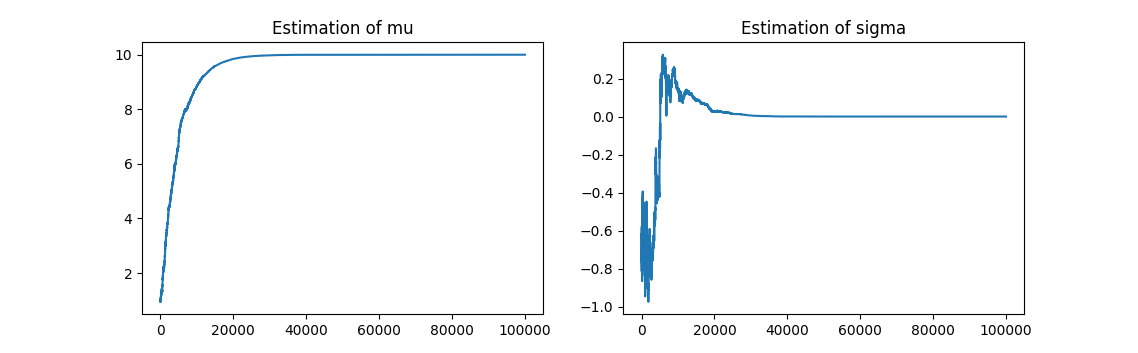
\includegraphics[scale=0.5]{mu_and_sigma.png}
\end{figure*}


\newpage
\section{\normalsize 
For discrete MDP, Derive the following Bellman equation for action value function from its definition: $q_\pi(s,a) = \E\left[ G_t | S_t = s, A_t = a, A_k \sim \pi, \forall k > t \right]$, where $S_t$ is the state at $t$, $A_t$ is the action at $t$, $G_t$ is the return after $t$, $\pi$ is the policy, $\gamma$ is the discount factor, $r(s,a) = \sum_r r  \sum_{s'} p(s', r | s, a)$ and $p_\pi(s', a'|s, a) = \sum_r p(s', r| s, a)\pi(a'|s')$
 (5 points).
}
\begin{align}
q_\pi(s, a) = r(s, a) + \gamma \sum_{s', a'} p_\pi(s', a'|s, a) q_\pi(s', a').
\end{align}

\begin{align*}
	q_\pi(s,a) &= \E\left[ G_t | S_t = s, A_t = a, A_k \sim \pi, \forall k > t \right]\\
	&=\E_{\pi}\left[ G_t | S_t = s, A_t = a \right]\\
	&=\E_{\pi}\left[ R_t+\gamma G_{t+1} | S_t = s, A_t = a \right]\\
	&=\E\left[ R_t | S_t = s, A_t = a \right] +\gamma\E_{\pi}\left[ G_{t+1} | S_t = s, A_t = a \right]\\
	&=\sum_r r  \sum_{s'} p(s', r | s, a) + \gamma\E\left[ \E_{\pi}\left[G_{t+1}|S_{t+1}, A_{t+1}\right] | S_t = s, A_t = a \right]\\
	&=r(s,a) + \gamma\E\left[ q_\pi(S_{t+1}, A_{t+1})| S_t = s, A_t = a \right]\\
	&=r(s,a) + \gamma\sum_{s',a'}\sum_r p(s', r| s, a)\pi(a'|s')q_\pi(s',a')\\
	&=r(s,a) + \gamma\sum_{s',a'}p_\pi(s', a'|s, a)q_\pi(s',a')\\
\end{align*}


%\vspace{7cm}
\section{\normalsize 
Write the above Bellman equation in matrix form
 (5 points).
}

\begin{align*}
	v_{\pi}(s) &= \sum_{a}{\pi(a|s)\sum_{s',r}{p(s',r|s,a)\big(r + \gamma v_{\pi}(s')\big)}}\\
	&= \sum_{a}{\pi(a|s)\sum_{s',r}{p(s',r|s,a)r}} + \gamma\sum_{a}{\pi(a|s)\sum_{s',r}{p(s',r|s,a)v_{\pi}(s')}}\\
	&= \sum_{a}{\pi(a|s)r(s,a)} + \gamma\sum_{s'}{\Big[\sum_{a}{\pi(a|s)p(s'|s,a)}\Big]v_{\pi}(s')}\\
	&= r_{\pi}(s) + \gamma \sum_{s'}{p_{\pi}(s'|s)v_{\pi}(s')}
\end{align*}

\begin{equation*}
\vpi = \rpi + \gamma \Ppi \vpi
\end{equation*}

\begin{equation*}
\begin{bmatrix}
v_{\pi}(s_0) \\
v_{\pi}(s_1) \\
\vdots
\end{bmatrix}
=
\begin{bmatrix}
r_{\pi}(s_0) \\
r_{\pi}(s_1) \\
\vdots
\end{bmatrix}
+ \gamma
\begin{bmatrix}
p_{\pi}(s_0|s_0) & p_{\pi}(s_1|s_0) & \dots \\
p_{\pi}(s_0|s_1) & p_{\pi}(s_1|s_1) & \dots \\
\vdots & \vdots & \ddots
\end{bmatrix}
\begin{bmatrix}
v_{\pi}(s_0) \\
v_{\pi}(s_1) \\
\vdots
\end{bmatrix}
\end{equation*}


\newpage

\section{\normalsize 
Consider a policy $\pi$ that is not optimal, that is $v_\pi(s) < v_{\pi^*}(s), \exists s$. Also consider the greedy-policy operator $g$ that gives a policy $gq$ which is greedy with respect to a given function $q$, that is, $(g q)(s) = \arg\max_b q(s, b)$, assuming there is no tie. Show that, $v_{gq_\pi}(s) > v_\pi(s), \exists s$
 (5 points).
}

\begin{align*}
	v_\pi(s) &= \sum_a\pi(a|s)q_\pi(s,a)\\
	v_{gq_\pi}(s) &=\sum_a gq_{\pi}(a|s)q_\pi(s,a)\\
	&=q_\pi(s, \arg\max_bq_\pi(s,b))\\
	&=\max_a q_\pi(s,a)\\
	v_{gq_\pi}(s) =\max_a q_\pi(s,a) &\ge v_\pi(s) = \sum_a\pi(a|s)q_\pi(s,a), \forall s
\end{align*}
{\sol
The condition of equality under all states is that optimal policy, contradict

}
\en
$$
v_{gq_\pi}(s) > v_\pi(s), \exists s
$$

%\vspace{8cm}

\section{\normalsize 
As we have seen, the action value iteration method can be written as: $\q_{k+1} = \q_k - \alpha \left( \left({\bf I} - \gamma \bP_{g\q_k}  \right)\q_k - \br \right)$, where $\q$ is the estimate of action value in vector form, and the vector $\br$ contains $\left[ \br \right]_{sa} = r(s,a)$ for different $s,a$. Also, the matrix $\bP_{g \q_k}$ contains state-action-transition probabilities, $\left[ \bP_{g\q_k} \right]_{sa, s'a'} = p(s'|s, a) (g \q_k)(a'|s')$, where next actions are taken under policy $g \q_k$, which is the greedy policy with respect to $\q_k$.
Find the condition under which the action-value iteration method converges, and convince that the condition is satisfied in general.
 (5 points).
}

\begin{align*}
	\q_{k+1} &= \q_k - \alpha \left( \left({\bf I} - \gamma \bP_{g\q_k}  \right)\q_k - \br \right) \\
	&= \q_k, -\alpha\bf{I}\q_k - \alpha \gamma \bP_{g\q_k}\q_k -\alpha r\\
	&=\left(\bf{I} - \alpha\bf{I} - \alpha\gamma\bP_{g\q_k} \right)\q_k - \alpha r\\
	&\text{denote $A_k$ as $\left(\bf{I} - \alpha\bf{I} - \alpha\gamma\bP_{g\q_k} \right)$ and $b$ as $ \alpha r $ }\\
	&=A_k \q_k -b\\
	&=A_k(A_{k-1}\q_{k-1} - b) -b\\
	&=A_kA_{k-1}\q_{k-1} - A_kb - b\\
	&\cdots\\
	&=\prod_{t=0}^kA_t\q_0 - \sum_{t=0}^k \left[\prod_{j=i}^k A_j\right] b - b
\end{align*}
{\sol
The condition for convergence is $\lim_{k\to +\infty} \prod_{t=0}^k A_t \to \bf{0} $, which requires $\rho(A_t)=\rho(\bf{I} - \alpha\bf{I} - \alpha\gamma\bP_{g\q_t}) < 1, \forall t\in T$, where $\rho$ is the spectral radius. Next, we argue that this condition is satisfied in general. The above condition equals to $\rho\big(\alpha(\bf{I} - \gamma\bP_{g\q_t})\big) >0, \forall t \in T$ as the eigenvalue of $\bf{I}$ is 1. Based on the fact that $\bP_{g\q_t}$ is a Markov matrix whose eigenvalues are all less than or equal to 1, the condition required for $\rho\big(\alpha(\bf{I} - \gamma\bP_{g\q_t})\big) >0, \forall t \in T$ is $ \gamma < 1 $ and $ \gamma < 1 $ is usually satisfied in general.

}
\en


\newpage

\section{\normalsize 
Write the following state-value iteration method in matrix form: \\
$v_{k+1}(s) = v_k(s) + \alpha\left( \max_b \left[ r(s, b) + \gamma \sum_{s'} p(s'|s, b) v_{k}(s') \right] - v_k(s) \right)$
 (5 points).
}

\begin{align*}
	v_{k+1}(s) &= v_k(s) + \alpha\left( \max_b \left[ r(s, b) + \gamma \sum_{s'} p(s'|s, b) v_{k}(s') \right] - v_k(s) \right)\\
	&= (1-\alpha) v_k(s) + \alpha\left( \max_b \left[ r(s, b) + \gamma \sum_{s'} p(s'|s, b) v_{k}(s') \right] \right)\\
	&= (1-\alpha) v_k(s) + \alpha \max_b \left( q_k(s,b) \right) \\
	&= (1-\alpha) v_k(s) + \alpha \bP_{gq_k} q_k(s,b) \\
\end{align*}

\begin{equation*}
	v_{k+1}(s)= (1-\alpha) v_k(s) + \alpha \bP_{gq_k} q_k(s,b)
\end{equation*}

\begin{equation*}
\begin{bmatrix}
v_{k+1}(s_0) \\
v_{k+1}(s_1) \\
\vdots
\end{bmatrix}
= (1-\alpha)
\begin{bmatrix}
v_{k}(s_0) \\
v_{k}(s_1) \\
\vdots
\end{bmatrix}
+ \alpha
\begin{bmatrix}
p_{gq_k}(s_0, a_0|s_0) & p_{gq_k}(s_0, a_1|s_0) & \dots \\
p_{gq_k}(s_0, a_0|s_1) & p_{gq_k}(s_0, a_1|s_1) & \dots \\
\vdots & \vdots & \ddots
\end{bmatrix}
\begin{bmatrix}
q_{k}(s_0, a_0) \\
q_{k}(s_0, a_1) \\
\vdots
\end{bmatrix}
\end{equation*}

%\vspace{8cm}

\section{\normalsize 
Consider the two-state MDP example from lecture, where $\gamma=0.9$, reward $r(s,a)$ is 1 for state 1 and action 1, and zero for all other state action pairs, and the state transition probabilities $p(s'|s,a)$ are as follows: $p(0|0,0) = p(1|0,1) = p(0|1,0) = p(1|1,1)=1$, and zero for any other transition.
 (5 points). Now, consider a policy $\pi$ which takes action 0 at state 0 with probability 0.25 but takes the same action at state 1 with probability 0.75.
 Find $r_\pi(s) = \sum_a \pi(a|s)r(s,a)$, $p_\pi(s'|s) = \sum_a \pi(a|s)p(s'|s,a)$, and $v_\pi(s)$ for all $s$ and $s'$.
Mention the method you used for finding $v_\pi$ or show calculation.
 (5 points).
}

\begin{align*}
	r_\pi(0) &= \pi(0|0) * r(0,0) + \pi(1|0)*r(0,1) 
	= 0.25 * 0 + 0.75 * 0 = 0\\
	r_\pi(1) &= \pi(0|1) * r(1,0) + \pi(1|1)*r(1,1) 
	= 0.75 * 0 + 0.25 * 1 = 0.25\\
	p_\pi(0|0) &= \pi(0|0)*p(0|0,0) + \pi(1|0)*p(0|0,1)
	=0.25 * 1 + 0.75 * 0 = 0.25\\
	p_\pi(1|0) &= 1 - p_\pi(0|0) = 0.75\\
	p_\pi(0|1) &= \pi(0|1)*p(0|1,0) + \pi(1|1)*p(0|1,1)
	=0.75 * 1 + 0.25 * 0 = 0.75\\
	p_\pi(1|1) &= 1 - p_\pi(0|1) = 0.25
\end{align*}

{\sol
with $p$ and $r$, we can write $v_\pi$ in the matrix form $\vpi = \rpi + \gamma \Ppi \vpi$ and solve the linear system to obtain $v_\pi$:

}
\en

\begin{equation*}
\begin{bmatrix}
v_{\pi}(0) \\
v_{\pi}(1) \\
\end{bmatrix}
=
\begin{bmatrix}
r_{\pi}(0) \\
r_{\pi}(1) \\
\end{bmatrix}
+ \gamma
\begin{bmatrix}
p_{\pi}(0|0) & p_{\pi}(1|0) \\
p_{\pi}(0|1) & p_{\pi}(1|1) \\
\end{bmatrix}
\begin{bmatrix}
v_{\pi}(0) \\
v_{\pi}(1) \\
\end{bmatrix}
\end{equation*}

{\sol
	solve $\vpi = (\bf{I}-\gamma\Ppi)^{-1}\vpi$, we have $v_\pi(0) \approx 1.16, v_\pi(1) \approx 1.34$
	
}
\en

\newpage
\section{\normalsize 
For the same MDP, find $q_\pi$, mention the method you used for finding $q_\pi$ or show calculation, and describe $g q_\pi$, that is the greedy policy over $q_\pi$ for the policy $\pi$ described in the previous question
 (5 points).
}

\qquad Similar to Q16, we can obtain the matrix form of $ q_\pi $ and solve the linear system
\begin{align*}
	q_\pi(s,a) &= \sum_{s',r}p(s',r|s,a)\left[r+\gamma\sum_{a'}\pi(a'|s')q_\pi(s',a')\right] \\
	&=\sum_{s',r}p(s',r|s,a) r +  \gamma\sum_{s',r}p(s',r|s,a)\sum_{a'}\pi(a'|s')q_\pi(s',a')\\
	&=\sum_{r}p(r|s,a) r +  \gamma\sum_{s'}\sum_{a'}\pi(a'|s')p(s'|s,a)q_\pi(s',a')\\
	&=r(s,a) + \sum_{a', s'}p_\pi(s',a'|s,a)q_\pi(s',a')
\end{align*}
\begin{equation*}
q_\pi = \rpi + \gamma \Ppi q_\pi
\end{equation*}
\begin{equation*}
\begin{bmatrix}
q_{\pi}(0,0) \\
q_{\pi}(0,1) \\
\vdots
\end{bmatrix}
=
\begin{bmatrix}
r_{\pi}(0,0) \\
r_{\pi}(0,1) \\
\vdots
\end{bmatrix}
+ \gamma
\begin{bmatrix}
p_{\pi}(0,0|0,0) & p_{\pi}(0,1|0,0) & \dots \\
p_{\pi}(0,0|0,1) & p_{\pi}(0,1|0,1) & \dots \\
\vdots & \vdots & \ddots
\end{bmatrix}
\begin{bmatrix}
q_{\pi}(0,0) \\
q_{\pi}(0,1) \\
\vdots
\end{bmatrix}
\end{equation*}
fix the matrix

thus $ q_\pi = (\bf{I} - \gamma\Ppi)^{-1} + r_\pi $, the solutions are: .....


%\vspace{8cm}

\section{\normalsize 
Consider the nonlinear function approximator for supervised regression $Y \approx {\bf \theta}^\top \phi({\bf W}\x)$, where $Y$ is the target scalar output, $\x$ is the vector input, ${\bf \theta}$ is the output weight vector, $\bf W$ is the input weight matrix, and $\phi$ is the element-wise activation function for the hidden layer. Consider the activation function to be sigmoid.
Show the backpropagation update for input weights for this case in matrix form.
 (5 points).
}

{\sol
As this is a regression problem, we use Mean Squared Error $  \left( Y - {\bf \theta}^\top \phi({\bf W}\x)\right)^2$as the objective:

}
\en



\begin{align*}
	\theta_{t+1} &= \theta_t - \alpha_t \nabla_{\theta_t}(Y_t - \theta^\top \phi({\bf W}_t\x_t))^2\\
	&= \theta_t + 2 \alpha_t (Y_t - \theta^\top \phi({\bf W}_t\x_t))\phi({\bf W}_t\x_t)\\
	\\
	{\bf W}_{t+1} &= {\bf W}_t - \alpha_t \nabla_{{\bf W}_t}(Y_t - \theta^\top \phi({\bf W}_t\x_t))^2\\
	&= \theta_t + 2 \alpha_t (Y_t - \theta^\top \phi({\bf W}_t\x_t))\nabla_{{\bf W}_t}\phi({\bf W}_t\x_t)\\
	&= \theta_t + 2 \alpha_t (Y_t - \theta^\top \phi({\bf W}_t\x_t))\phi({\bf W}_t\x_t)\circ(1-\phi({\bf W}_t\x_t))\nabla_{{\bf W}_t}{\bf W}_t\x_t\\
	&= \theta_t + 2 \alpha_t (Y_t - \theta^\top \phi({\bf W}_t\x_t))\phi({\bf W}_t\x_t)\circ(1-\phi({\bf W}_t\x_t))\x_t^\top\\
	& \text{ where $\circ$ indicates elementwise multiplication}
\end{align*}




\end{document}





